\chapter{Tracking Examples} \label{Exam}

A simple tracking example is shown with its input file (~\ref{input}),
its output file (~\ref{output}) and some corresponding plots in
(~\ref{plots}).

\section{Input Example} \label{input}

For the description of the different input blocks see
chapter~\ref{InpStr}.

\begin{figure}[H]
\begin{center}
  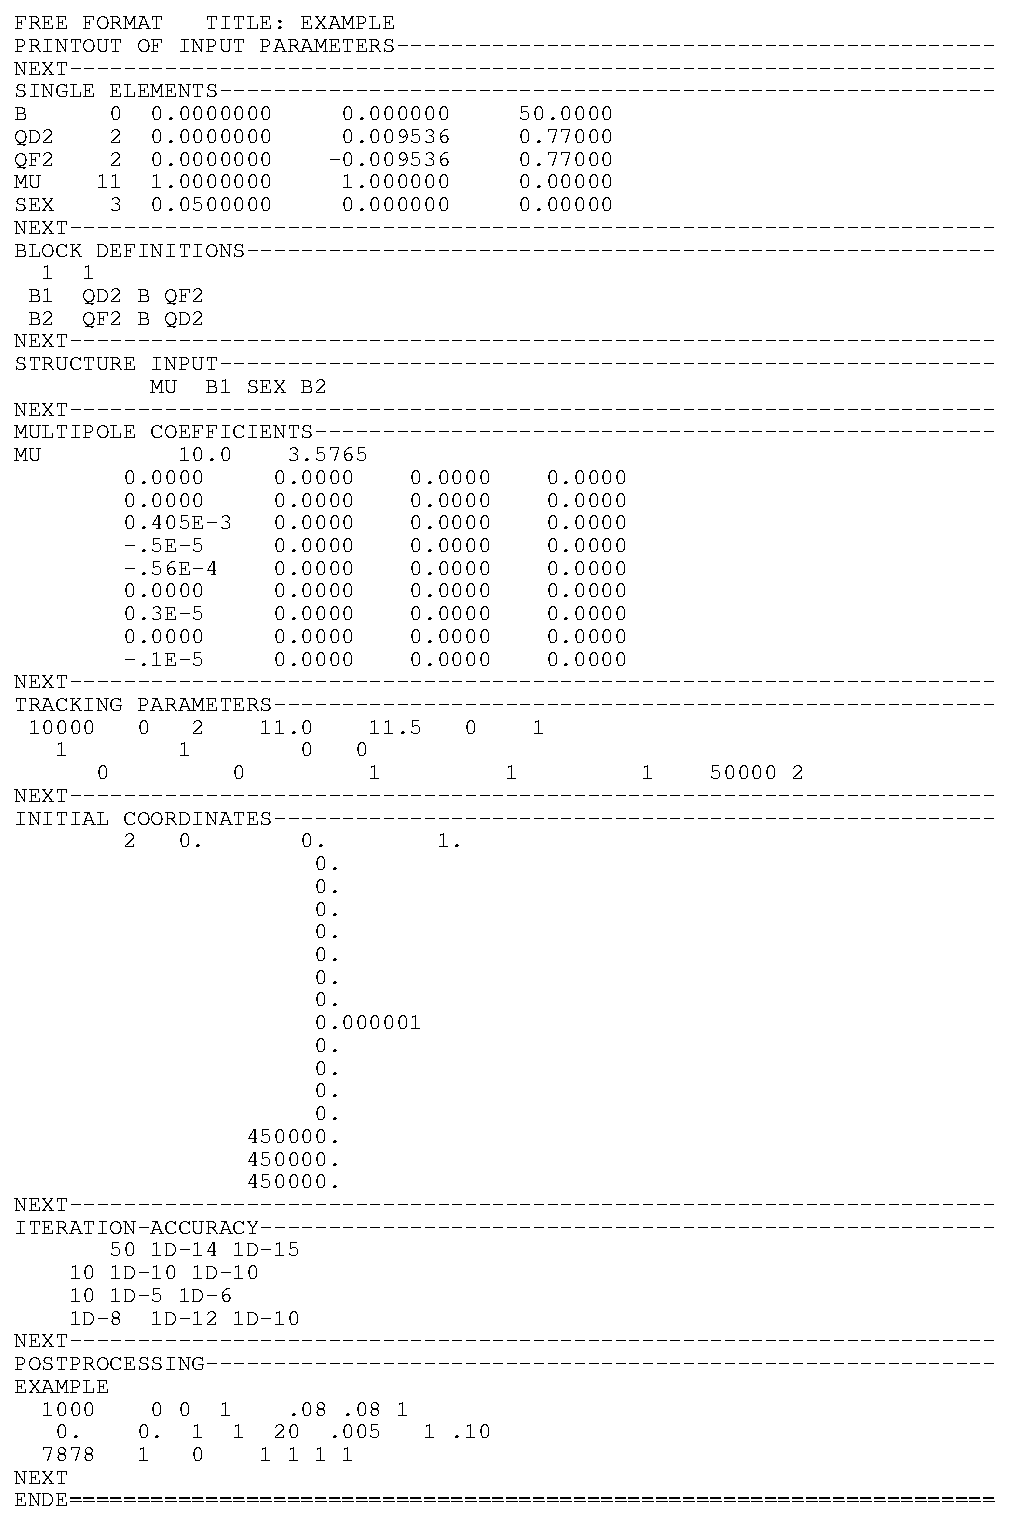
\includegraphics[width=16cm,height=18cm]{expout1}
\end{center}
\end{figure}

\clearpage

\section{Output Example} \label{output}

The preprocessing part is shown first.
\begin{figure}[H]\vspace{-5mm}
\begin{center}
  \mbox{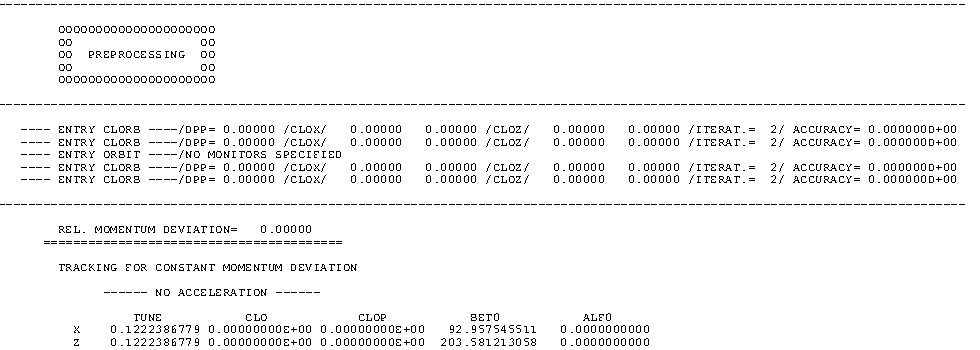
\includegraphics[width=16cm,height=6.5cm]{expout2}}
\end{center}
\end{figure}
Followed by the initial coordinates and the final coordinates for a
regular (right side) and chaotic (left side) case.
\begin{figure}[H]\vspace{-5mm}
\begin{center}
  \mbox{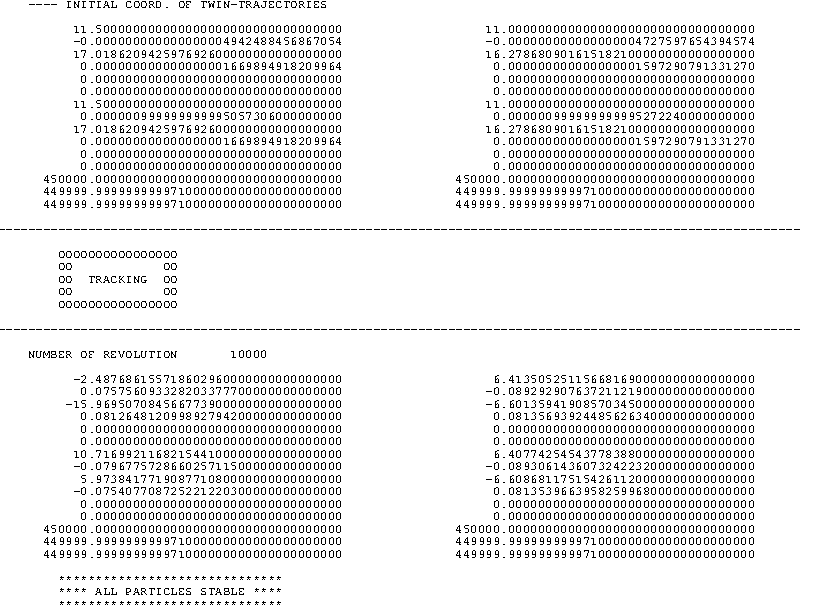
\includegraphics[width=16cm,height=13cm]{expout3}}
\end{center}
\end{figure}

\clearpage

Finally part of the post--processing for the two particles are shown
(chaotic on the left and regular on the right respectively) and a
summary of the post--processing is given.
\begin{figure}[H]
\begin{center}
  \mbox{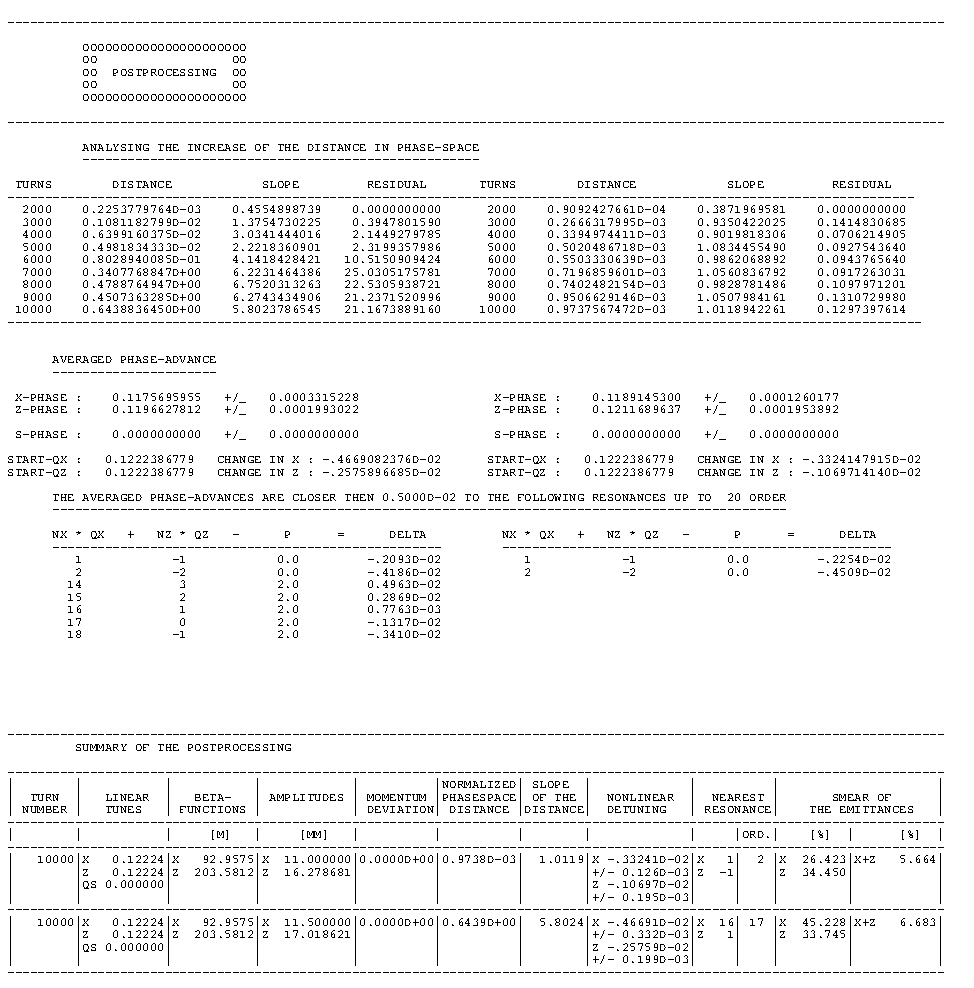
\includegraphics[width=16cm,height=21cm]{expout4}}
\end{center}
\end{figure}

\clearpage

\section{Plot Example} \label{plots}

{\small In figure~\ref{Lya} a typical example of the evolution of the
  distance in phase space is shown of a regular and chaotic particle.
  Figure~\ref{H-proj} and figure~\ref{P-proj} show the corresponding
  horizontal phase space and the physical phase space projections
  respectively. An example of the stroboscoped phase space is shown in
  figure~\ref{P-stro}, where the motion in the chaotic case is beyond
  a ``separatrix'' in the four--dimensional phase space. Even in the
  FFT (figure~\ref{P-FFT}) one can see the effect of chaotic
  behaviour: it leads to a widening of the lines of the spectrum.}
\begin{figure}[H] \vspace*{-5mm}
\begin{center}
  \mbox{\includegraphics*[width=9.cm]{exp1}}
  \\[5mm]
  \mbox{\includegraphics*[width=9.cm]{exp9}}
 \caption{\small Evolution of the Distance of Phase Space for Regular
   \mbox{(upper part)} and Chaotic \mbox{(lower part)} Motion.}
 \label{Lya}
\end{center}
\end{figure} 

\begin{figure}[H]
\begin{center}
  \mbox{\includegraphics*[width=10.5cm]{exp2}}
  \\[5mm]
  \mbox{\includegraphics*[width=10.5cm]{exp10}}
 \caption{Horizontal Phase Space Projections for the
   Regular (upper part) and the Chaotic \mbox{(lower part)} Cases.}
 \label{H-proj}
\end{center}
\end{figure}

\begin{figure}[H]
\begin{center}
  \mbox{\includegraphics*[width=10.5cm]{exp4}}
  \\[5mm]
  \mbox{\includegraphics*[width=10.5cm]{exp12}}
 \caption{Physical Phase Space Projections for the Regular
   \mbox{(upper part)} and the Chaotic \mbox{(lower part)} Cases.}
 \label{P-proj}
\end{center}
\end{figure}

\begin{figure}[H]
\begin{center}
  \mbox{\includegraphics*[width=10.5cm]{exp6}}
  \\[5mm]
  \mbox{\includegraphics*[width=10.5cm]{exp14}}
 \caption{\small{Stroboscoped Vertical Phase Space Projections
     for the Regular (upper part) and the Chaotic (lower part) Cases
     respectively.  The regular motion stays inside a ``separatrix''
     with two unstable fix--points visible, while the chaotic motion
     is clearly outside this ``separatrix''.}}
 \label{P-stro}
\end{center}
\end{figure}

\begin{figure}[H]
\begin{center}
  \mbox{\includegraphics*[width=10.5cm]{exp7}}
  \\[5mm]
  \mbox{\includegraphics*[width=10.5cm]{exp15}}
 \caption{Horizontal FFT--Analysis for the Regular (upper part)
   and the Chaotic (lower part) Cases.}
 \label{P-FFT}
\end{center}
\end{figure}
